\documentclass{article} % For LaTeX2e
\usepackage{nips12submit_e,times}
%\documentstyle[nips12submit_09,times,art10]{article} % For LaTeX 2.09

\usepackage{amsmath} % loads AMS-Math package
\usepackage{euscript}
\usepackage{amssymb}
\usepackage{epsfig} % allows PostScript files
\usepackage{graphicx}
\usepackage{caption}
\usepackage{subcaption}
\usepackage{color}
\usepackage{multirow}
%\usepackage{url}
\usepackage{hyperref}
\newcommand{\tr}{^{\rm T}}

\newcommand{\alex}[1]{\textcolor{red}{#1}}


\title{Tracked Feature Outlier Detection}


\author{
Nicolas Feltman\\
Department of Computer Science\\
Carnegie Mellon University\\
Pittsburgh, PA 15213 \\
\texttt{nfeltman@cs.cmu.edu} \\
\And
Alex Beutel\\
Department of Computer Science\\
Carnegie Mellon University\\
Pittsburgh, PA 15213 \\
\texttt{abeutel@cs.cmu.edu} 
}

% The \author macro works with any number of authors. There are two commands
% used to separate the names and addresses of multiple authors: \And and \AND.
%
% Using \And between authors leaves it to \LaTeX{} to determine where to break
% the lines. Using \AND forces a linebreak at that point. So, if \LaTeX{}
% puts 3 of 4 authors names on the first line, and the last on the second
% line, try using \AND instead of \And before the third author name.

\newcommand{\fix}{\marginpar{FIX}}
\newcommand{\new}{\marginpar{NEW}}

\nipsfinalcopy % Uncomment for camera-ready version

\begin{document}


\maketitle

\begin{abstract}
In this project, we employ a naive Bayes Gaussian mixture model to detect outliers in a set of image-feature traces derived from SIFT and KLT analysis of unstable video data.  We identify two applications: 1) preprocessing data for standard structure-from motion algorithms, and 2) robust motion detection and isolation in presence of shakey video.  In the first application, we find improvement of up to 100\% in our decomposability metric for some scenes.  In the second application, we show a strong ability to disentangle scene motion from camera motion.
\end{abstract}


\section{Introduction} % (fold)
\label{sec:Introduction}

A common challenge in computer vision is accurately tracking features through a
video.
%Many computer vision algorithms build upon these tracked features, so
%accurately tracking the features and understanding the traces through time that
%the features produce is important.  
There has been much prior work on feature
selection (ie SIFT \cite{sift}), which focuses on finding features in an image
and picking out the ``best'' ones.  Important later work focused on matching
features between images and after that tracking features through a sequence of
frames in a video (ie KLT \cite{klt}).  
%These tools produce a trace of the features through space and time.
%Given these feature traces, researchers attempt to use them for
%numerous computer vision applications
Researchers have used such feature traces for numerous applications; we focus
on two: robust structure from motion and robust movement isolation.    

Structure from motion is a common application in which we attempt to recover
the structure of the objects in a scene based on the feature traces.  However,
incorrect feature traces worsen the results of the structure from motion
algorithm.  This became more problematic as SIFT and KLT had some difficulty
with shaky video, such as that produced from waving a mobile phone around.
We found that traces from moving objects in a scene also weakened the
results of the structure from motion algorithm.  Therefore, we sought to create
a model by which to separate these abnormal feature traces from the normal,
valid ones, with the ultimate goal of removing abnormal traces and improving
the structure from motion.  Our key insight, which we will explain in more
detail later, is that normal traces of static objects in a scene generally look
similar to one another since their trace is almost entirely based on the motion
of the camera, where as the bad traces and traces of moving objects look very
different.  Therefore, we created a model to compare trace shapes and detect
outliers.

As we produced this model, we found it was excellent at detecting moving
objects in a scene, regardless of camera motion.  We decided to apply our
outlier detection model to robustly isolating motion in shaky video.  Given an
``outlier score'' from our previous model we create a secondary model to
estimate if a given pixel in a given frame of video is of a moving object or a
static object, based on the traces around that pixel and their scores.  With
this model we can construct a video containing only the moving elements in the
video and removing background pixels.

In Section \ref{sec:background} we give a brief background on the computer
vision research that we build upon, such as SIFT, KLT, and structure from
motion.  In Section \ref{sec:formulation} we more precisely formulate the
problem and describe our model for outlier detection.  In Section \ref{sec:sfm}
we describe the application of our model to the problem of robust structure
from motion, and in Section \ref{sec:motion} we describe the application of our
model to the problem of robust motion isolation.  For each application we run
our algorithm on numerous videos, some taken by us with mobile phones and
others downloaded from YouTube, and analyze the results.


% section Introduction (end)

\section{Background}
\label{sec:background}

Our method is built on top of the SIFT \cite{sift} feature selector and KLT
\cite{kltImpl,klt} feature matching algorithm.  These were chosen because
they meet a minimum level of performance required to illustrate our method, and
stable implementations of both are freely available.  The SIFT algorithm is
generally desirable because it is invariant to changes in scale and lighting,
as well as small changes in viewing angle.  The former properties may not be
necessary given our particular application, and so investigation into other
feature selectors could reasonably improve our implementation.  While the KLT
matching algorithm is generally robust, it has the drawback of only returning
features represented in every input frame.  In practice, this is only a problem
when the video includes a ``bad frame'' (eg. one frame is extremely blurry)
which scrambles all feature tracking.

One of our applications builds on structure from motion \cite{sfmImpl,sfm}, in
which the task is to use the projection of a labeled set of three-dimensional
points from several viewpoints (``frames'') to recover (1) the true location of
the points in 3D space, and (2) the location and direction of the camera for
each frame.  In order to support our work, we will cover some of the exposition
of \cite{sfm}. One key simplifying assumption in structure from motion is
orthography, that points are projected orthographically onto the plane of the
camera.  Firstly, note that the centroid of a set of points commutes with
orthographic projection of those points onto some plane.  Where $p_1, \ldots,
p_P$ is a series of points in three dimensional space, and $A$ is any $2\times
3$ orthogonal projection matrix:
\begin{align}
	{\it centroid}({\it project}_A (\{p_1, \ldots, p_P\})) = A[p_1 \ldots p_P]\left[\begin{array}{c}1/P \\ \vdots \\ 1/P\end{array}\right] ={\it project}_A({\it centroid} (\{p_1, \ldots, p_P\}))
	\end{align}
This implies that we can correct for camera translation by normalizing every
frame to the centroid of its points, thereby leaving only the effects of
projection onto the camera plane.  Having done this, let
$A_1$,$A_2$,\ldots,$A_F$ be the series of $2\times 3$ orthogonal projection
matrices through time.  Thus a single 3D point $p$ will take the path $A_1p$,
$A_2p$, \ldots, $A_Fp$ in normalized screen space.  Considering this across a
whole set of normalized points $p_1$, $p_2$, \ldots, $p_P$, we get a grand
matrix, $D$, of all data.  This can be factored into two separate matrices, one
corresponding to the direction of the camera and the other to the collection of
points:
\begin{align}\label{decomp}
	D=
	\left[ \begin{array}{cccc} 
		A_1p_1 & A_1p_2 & \cdots & A_1p_P \\
		A_2p_1 & A_2p_2 & \cdots & A_2p_P \\
		\vdots & \vdots & \ddots & \vdots \\
		A_Fp_1 & A_Fp_2 & \cdots & A_Fp_P
	\end{array} \right ] = 
	\left[ \begin{array}{c} A_1 \\ A_2 \\ \vdots \\ A_F \end{array} \right ] \left[ \begin{array}{cccc} p_1 & p_2 & \cdots & p_P \end{array} \right ]
	\end{align}
Since the sizes of these factors are $2F \times 3$ and $3 \times P$, we know
that the original $D$ matrix, absent of any measurement noise, has rank three.  Of
course, there is more than one way to form the decomposition in Equation
\ref{decomp}; extra constraints come from restrictions on the projection
matrices, and remaining freedom is attributable to freedom of axis choice.
Details of the computation can be found in \cite{sfm}.  For our purposes, the
important detail is that $D$ is rank three.


\section{Problem Formulation and Learning Model}

\begin{figure}[h]
	\begin{center}
		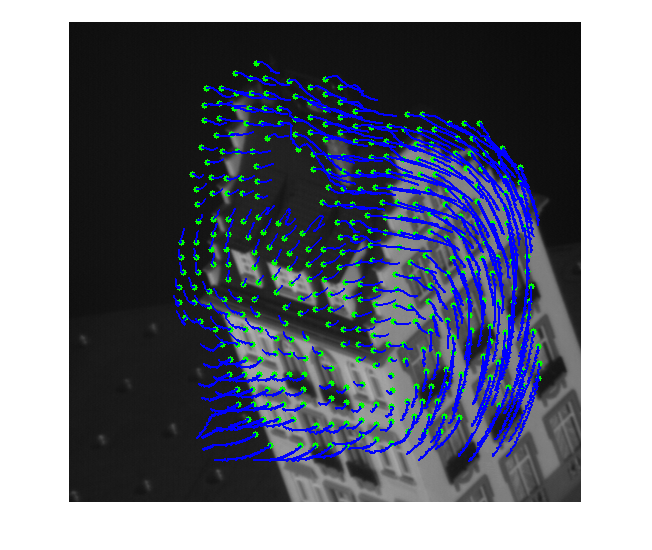
\includegraphics[width=2.5in]{figs/hotel-traces.png}
	\end{center}
	\caption{Example of traces from SIFT and KLT}
	\label{fig:traces}
\end{figure}


We use SIFT features and the KLT matching algorithm to track a set of features
through time.  The particular parameters of the tracking and matching phases
depend on application.  Our learning algorithm operates directly on the output
of KLT.  The features are represented as a set of $P$ feature traces across $F$
frames where each trace comprises two $F\times 1$ vectors,
\begin{align*}
x = (x_1, \ldots, x_F)\tr && y = (y_1, \ldots, y_F)\tr
\end{align*}
which together trace out the screen-space location of tracked points.  
In Figure \ref{fig:traces}, we see an example of overlaying the traces from KLT
on the first image in a sequence.  As was mentioned previously, our goal is
detect traces that are outliers.  We define outliers to be traces whose {\it
shape} is largely different than the shape of the other traces in the image.
For example, in Figure \ref{fig:colored-traces}(a), we note that some traces,
such as the red ones on the carpet, look quite different from the traces on the
chair.

Therefore, in order to compare trace shape we compare the velocity of the
tracked features at given points in time.
%We are not interested in the location of tracked features as much as their velocity at
%given points in time, which corresponds to the shape of the traces.  
This differential is recovered by finding the movement of each point relative
to the previous frame:
\begin{align*}
\dot x = (x_2-x_1, \ldots, x_F-x_{F-1})\tr && \dot y = (y_2-y_1, \ldots, y_F-y_{F-1})\tr
\end{align*}
We assume in our model that motion of each trace is independent in its two
axes, and that the motions at any two points in time are independent.  This
assumption is highly reasonable for traces resulting from the unsteadiness of a
handheld camera, and is necessarily true if fast twitch motions occur within
the sampling frequency of the camera.  Thus, for each tracked feature point, we
can form a $2(F-1)\times 1$ vector, called the {\it trace differential vector}:
\begin{align*}
\dot w = \left( \begin{array}{c}\dot x \\ \dot y\end{array} \right)
\end{align*}
Once we've calculated the trace differential vectors, $\{\dot w_1, \dot w_2,
\ldots , \dot w_P\}$, for each of $P$ tracked points, we need a model to
differentiate ``normal'' and outlier traces.
Noting that it's possible for the set of valid traces to be split into several
distinct clusters (for example, the different faces of an object or different
objects in a scene), we decided to use a mixture model.  Because of the
aforementioned independence assumptions, a naive Bayes Gaussian mixture model (GMM)
is sufficient.  
Once we have trained our GMM, we can ``score'' each trace differential, giving it a
probability of being part of any mixture in the GMM.  We use the
log-probability from the trace differential as an indicator of the likelihood
that any given trace is an outlier.  This relatively simple model and the
resulting probabilities turn out to be quite useful for a number of tasks.

%train some sort of
%statistical model on the entire set.  With the trained model, we calculate the
%log-probability of each trace differential vector and interpret that as an
%outlier-score for the feature trace, with lower scores corresponding to more
%likely outliers.  The question then remains what sort of model to use.  
%Noting that it's possible for the set of valid traces to be split into several
%distinct clusters (for example, those correspondnig to different faces of an
%object), we decided to use a mixture model.  Because of the aforementioned
%independence assumptions, a naive bayes gaussian mixture model is sufficient.  

Having implemented this exact model on one of the homework assignments, we
decided to avoid numerical precision risks and use MATLAB's implementation,
which employs the expectation maximization algorithm.  In all of our
experiments, four mixture elements seems to produce reasonable results,
although this number might benefit from tweaking.  For stability reasons, a
small amount of regularization on the variance parameter is also required.
Since the resulting score of the model is very sensitive to the random
initialization of expectation maximization, we perform the entire train/score
sequence many times, and average the results in log-space.  In our experiments,
100 iterations averaged was sufficiently fast and produced little variance in score
between runs.


\section{Robust Structure From Motion}
\label{sec:sfm}

Given our Gaussian mixture model, we can now detect the similarity between
traces and use this probability to remove traces that decrease the quality of
performing structure from motion.  We first describe the application of our GMM
model to this problem, and then describe the setup and results of our
experiments.

\subsection{Model Application} % (fold)
\label{sub:Model Application}

In structure from motion, we focused on recovering the structure of a
static scene from a (possibly noisy) mobile camera.  We used our mobile phones,
an iPhone and Android, to collect data and found that unlike much original
research in the field, using an mobile phone by hand to capture video resulted
in highly unstable, shaky video.  The structure from motion algorithm works
fine with shaky video, but we found that SIFT and KLT often, as a result of
shaky, low-quality video, incorrectly traced features resulting in bad traces
and worsening the results for structure from motion.  Additionally, we found
that if there was a moving object in the video frame, it made it difficult for
the structure from motion algorithm to disentangle the motion of the object in
the scene from the motion of the camera, again worsening the results of the
structure from motion algorithm.  Sighting these two issues, we aimed to use or
GMM to improve the results of the structure from motion algorithm.

As explained previously, our GMM detects how similar traces are within a given
scene.  As a result, ``bad traces'' from incorrectly tracing a feature are
considered low probability traces since they are shaped quite differently from
correct traces matching the motion of the camera.  Similarly, moving objects in
a scene create create traces very different than those from static objects,
thus also giving them a low probability in our GMM.  When plotting a
distribution of these traces, as seen in Figure \ref{fig:logpdfs}, we see that
a relatively small percentage of the traces have a much lower probability than
a majority of the traces, which are of similar probability.  We consider this
segment of much lower probability traces to be outliers and thus should be
removed before performing the structure from motion algorithm.

\begin{figure}[h]
	\begin{subfigure}[b]{0.5\textwidth}
		\centering
		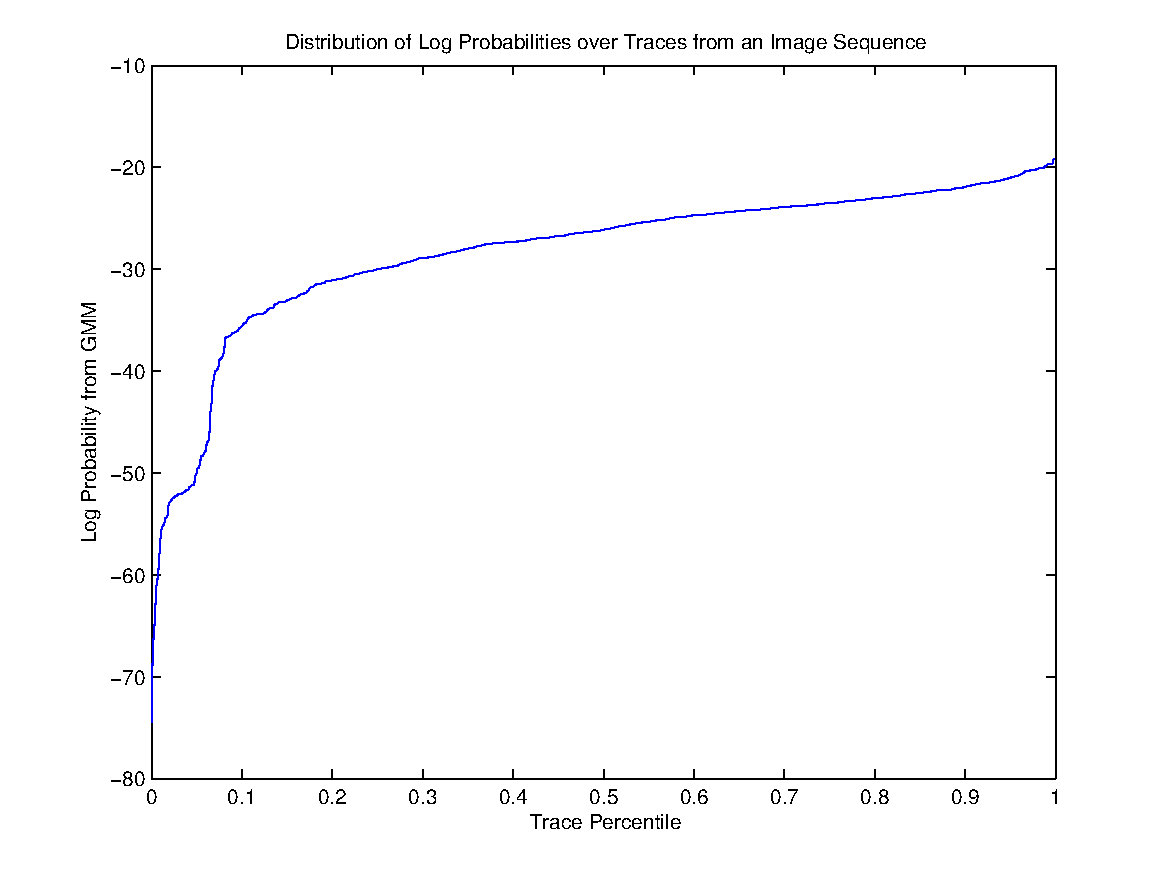
\includegraphics[width=0.9\textwidth]{figs/logpdfs-frame90.pdf}
		\caption{Outdoor dataset}
		\label{fig:logpdfs:90}
	\end{subfigure}%
	\begin{subfigure}[b]{0.5\textwidth}
		\centering
		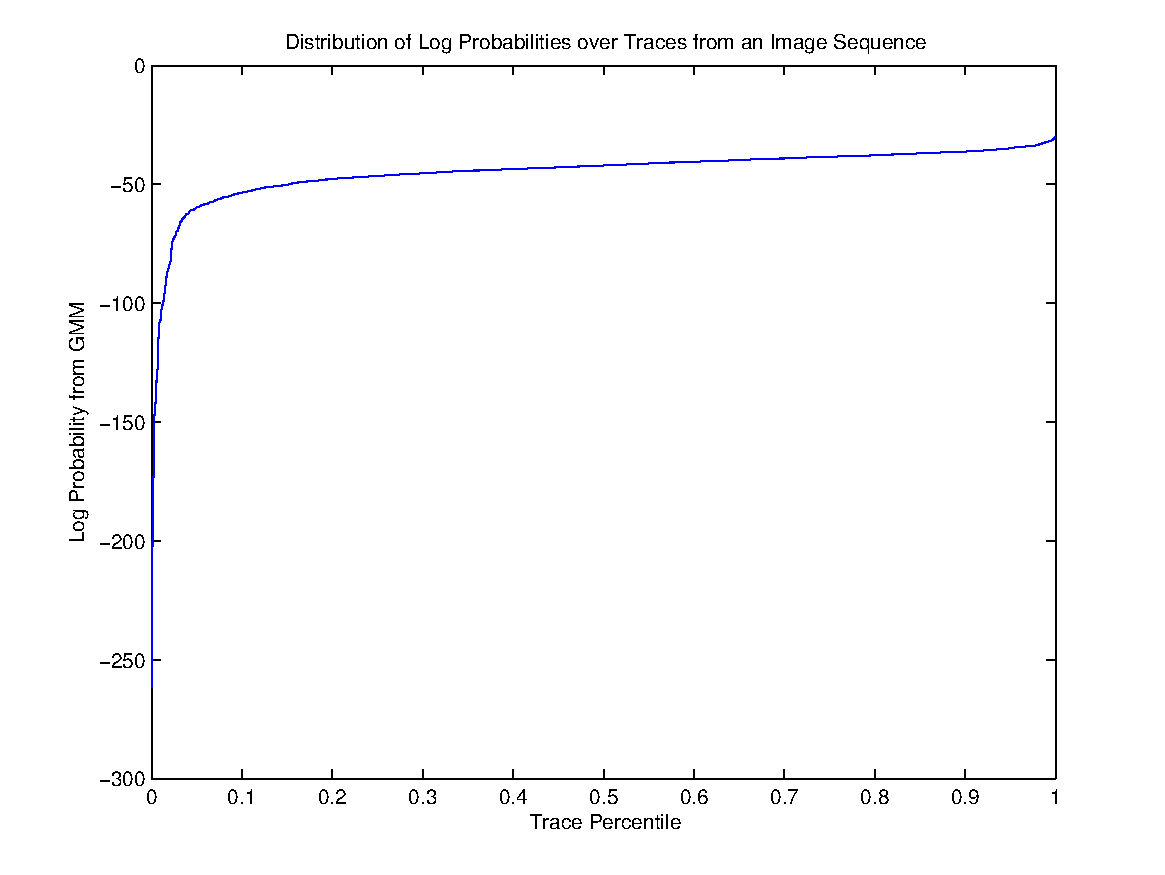
\includegraphics[width=0.9\textwidth]{figs/logpdfs.pdf}
		\caption{Outdoor dataset 2}
		\label{fig:logpdfs:105}
	\end{subfigure}%

	%\begin{center}
		%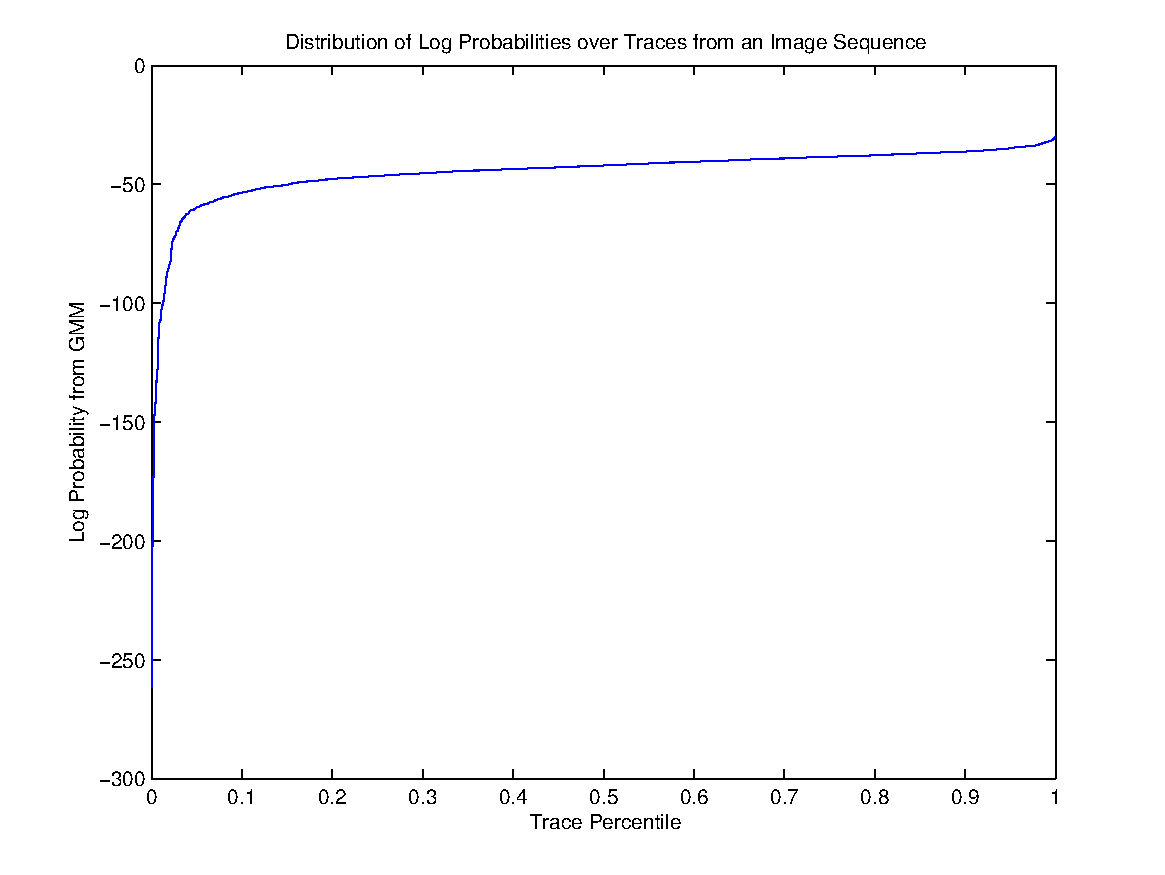
\includegraphics[width=4in]{figs/logpdfs.pdf}
	%\end{center}
	\caption{Distribution of log-probabilities generated by GMM for a set of traces in our ``Outdoor'' datasets}
	\label{fig:logpdfs}
\end{figure}

In our tests we found that approximately 10\% of traces were outliers, and thus
for simplicity using a simple thresholding mechanism, keeping only the top 90\%
of traces (based on their GMM score).  It is clear from the log probability
distributions from many videos, that our GMM generally produces distributions
similar to that in Figure \ref{fig:logpdfs}.  In future work, a more robust
method could be used to detect the change in log probability over trace
percentile and thus automatically find at what percentile is the ``best''
threshold.

% subsection Model Application (end)

\subsection{Experiments} % (fold)
\label{sub:Experiments}

\paragraph{Setup} 
To test our algorithm ran it on subsets of frames from multiple different data
sets: a desk chair, a lounge chair, and an outdoors scene.  For each we took a
subset of frames from the video so that a large number of points were tracked
across all frames, before running our algorithm.  For the desk chair we used 30
frames that tracked 164 features, for the lounge chair we used 20 frames that
tracked 508 features, and for the outdoor scene we used 10 frames that tracked
784 features and later in the video 15 frames that tracked 1596 features (which
we will refer to as ``Outdoors 2'').  In each video we have a substantial
amount of camera motion around a generally static scene.

\alex{nico - please expand on rank 3 thing here and check the rest of the description:}\\
To evaluate the effectiveness of the structure from motion algorithm we compare
a ratio of singular values from the singular value decomposition.  In each case
we take the SVD of the $W$ matrix and analyze the singular values in the
resulting $\Sigma$ matrix, where $\sigma_i$ is the $i$-th singular value.
Because the scene is three dimensional, we expect the data to be rank three,
and therefore ideally $\sigma_i$ for $1 \leq i \leq 3$ to be large and $\sigma_i$ for $i
> 3$ to be very small.  We therefore denote the following ratio as the purity
score for a given $W$ as computed by the SVD:
\begin{align}
	{\rm Purity\ Score} &= \frac{\sigma_1}{\sum_{i > 3} \sigma_i}.
\end{align}
Because all $\sigma_i$ in the denominator should be small, the larger the
purity score, the more clean the data in $W$ is and the better the result of
structure from motion.

\paragraph{Results} 

To visually evaluate the effectiveness of our methodology, we looked at the
distribution of log-probabilities as was discussed previously in Figure
\ref{fig:logpdfs}, as well as overlaying the trace scores on a frame from the
video, as can be seen in Figure \ref{fig:colored-traces}.  In these figures, we
color traces across a spectrum based on each trace's GMM score.  Traces with
higher probability are colored green, and traces with lower probability are
colored red. 

In Figure \ref{fig:colored-traces}(a) and (b) we see that feature tracking
algorithm occasionally finds faulty traces when trying to track a feature along
the carpet.  In each case we see that the shape of the trace is largely
different than that of other traces in the scene.  In Figure
\ref{fig:colored-traces}(c), the algorithm notices that a man walked through
the middle of the scene while filming it.  As a result, his traces show his
motion as well as the camera motion and are largely different than the traces
from the static objects in the scene.  Our algorithm successfully detects this
and gives these traces a low probability through the GMM.

\begin{figure}[tb]
	\hspace{-0.6cm}
	\begin{minipage}[b]{0.5\linewidth}
		\centering
		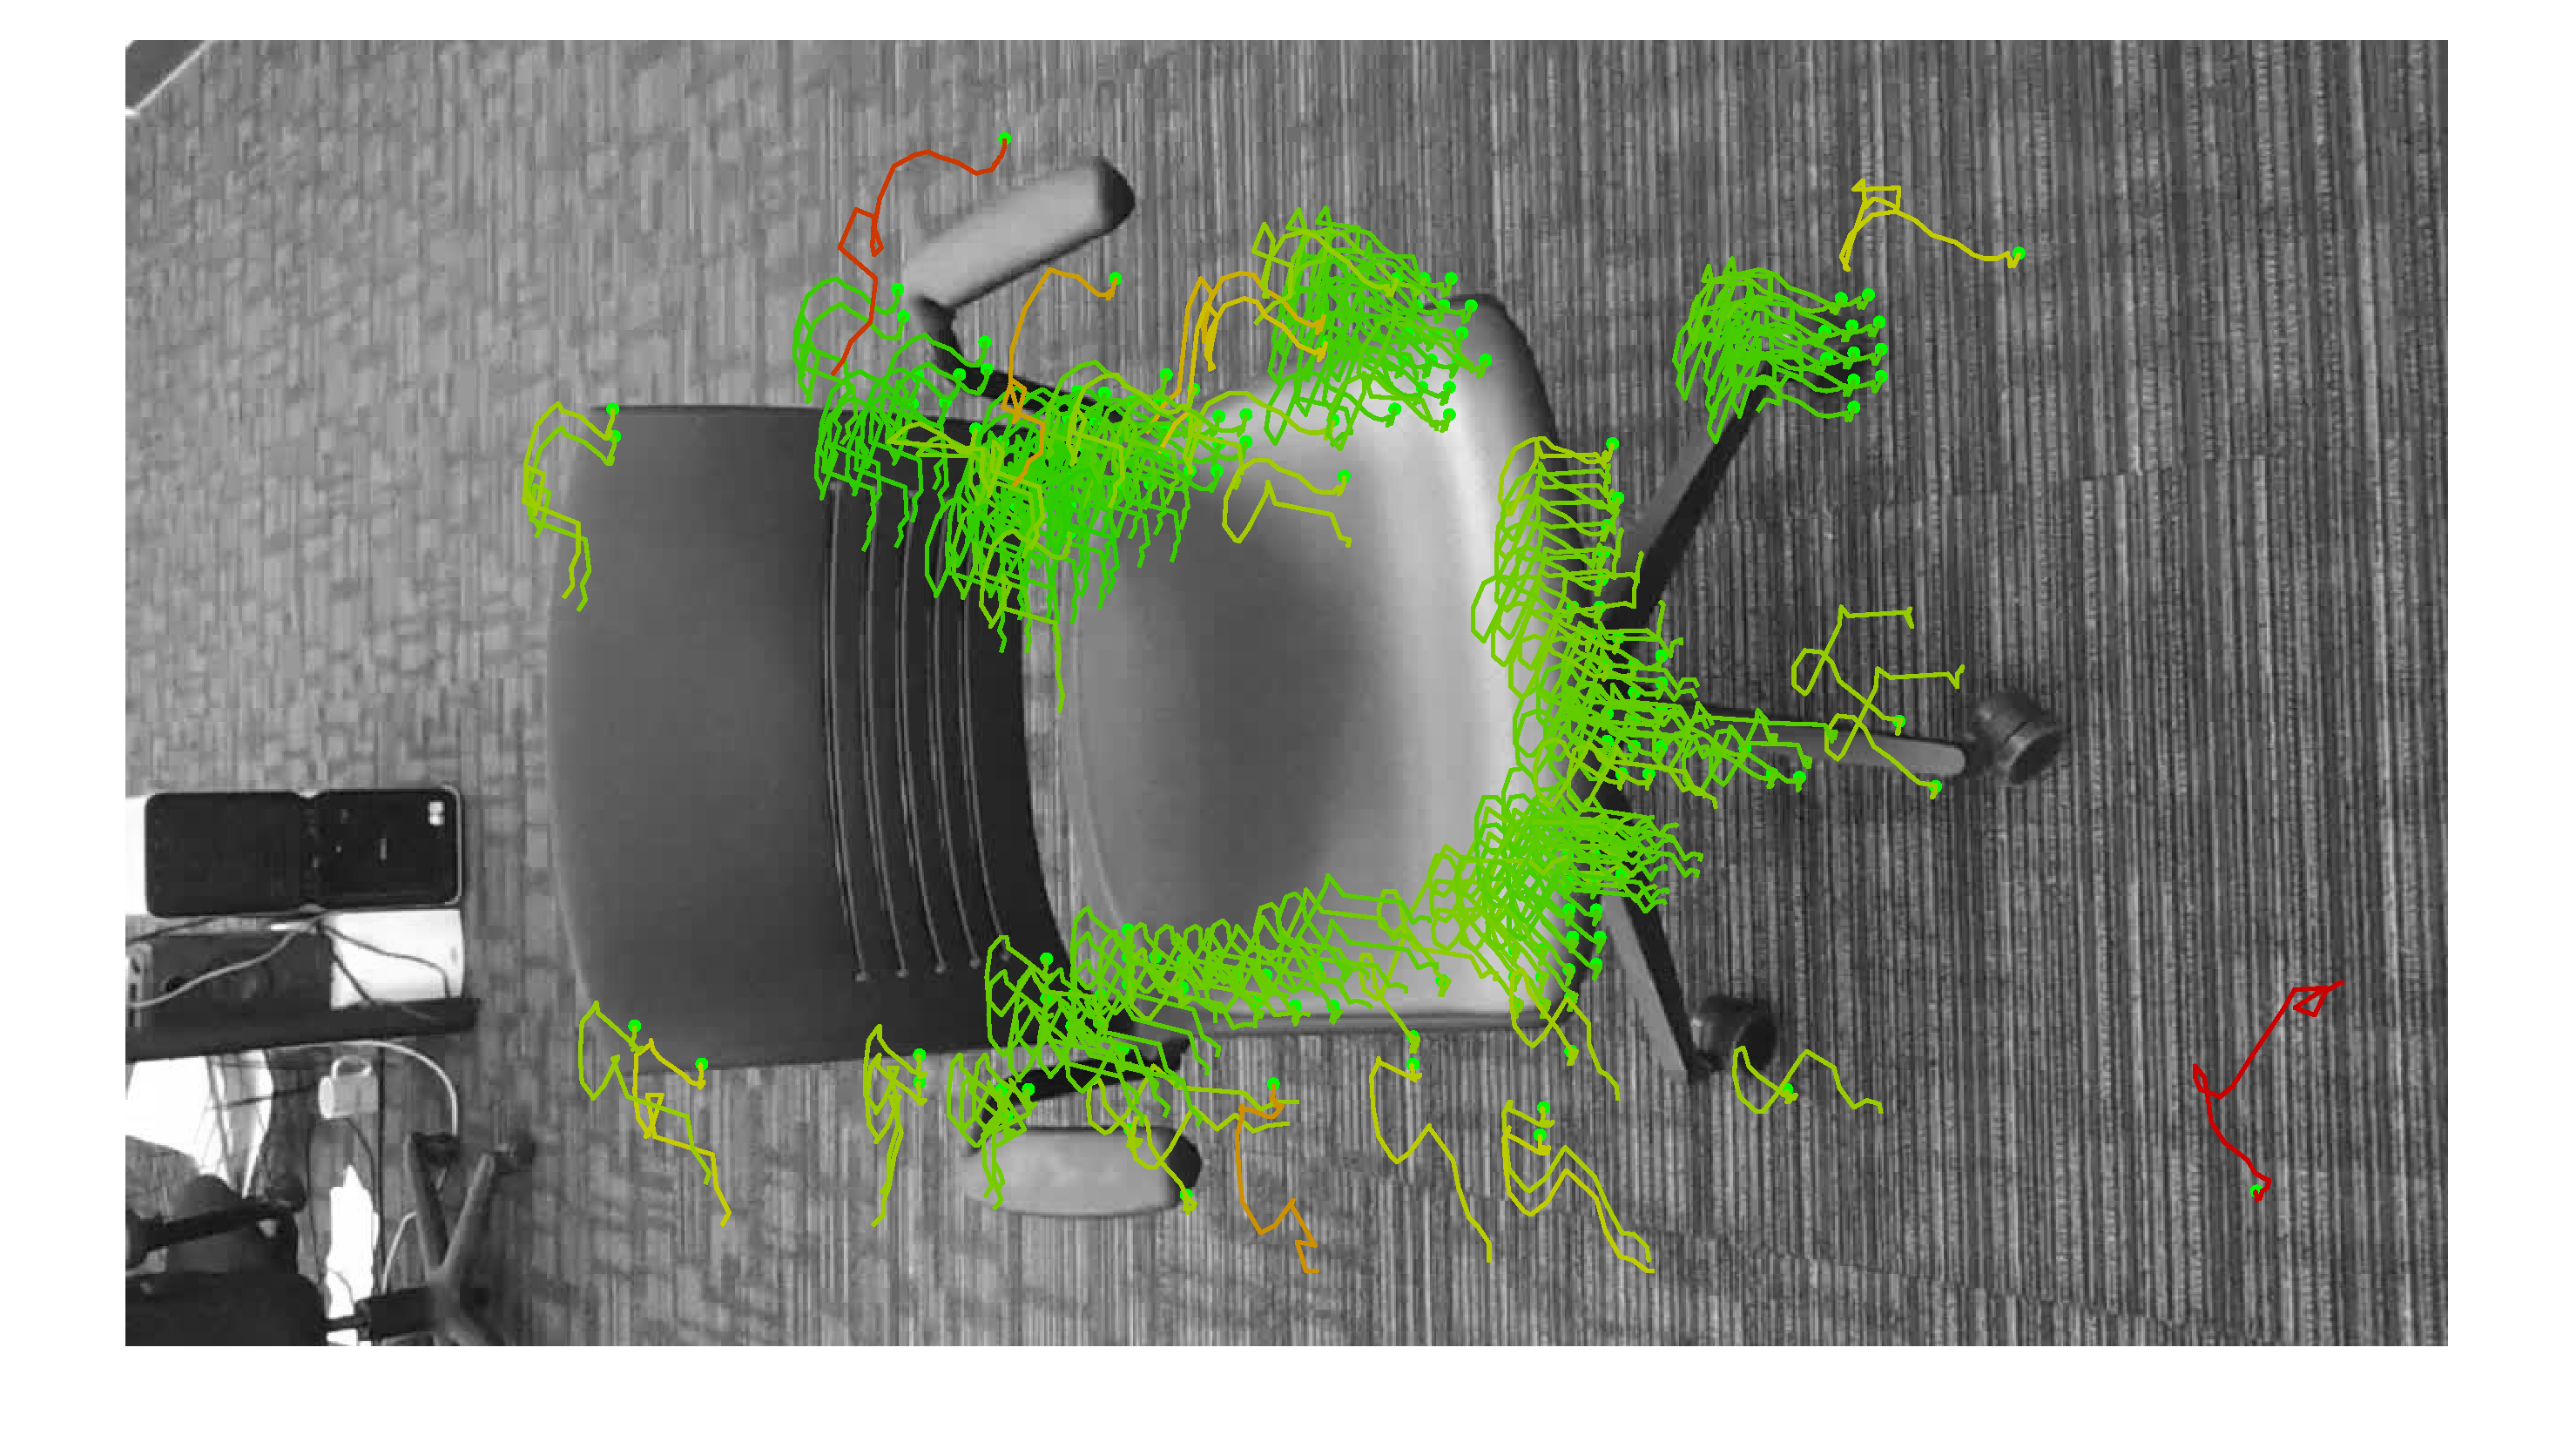
\includegraphics[height=2.1in,angle=-90]{figs/desk-1.pdf}\\ (a)
		%\caption{default}
	\end{minipage}
	\hspace{0cm}
	\begin{minipage}[b]{0.5\linewidth}
		\centering
		\begin{minipage}[b]{\linewidth}
			\centering
			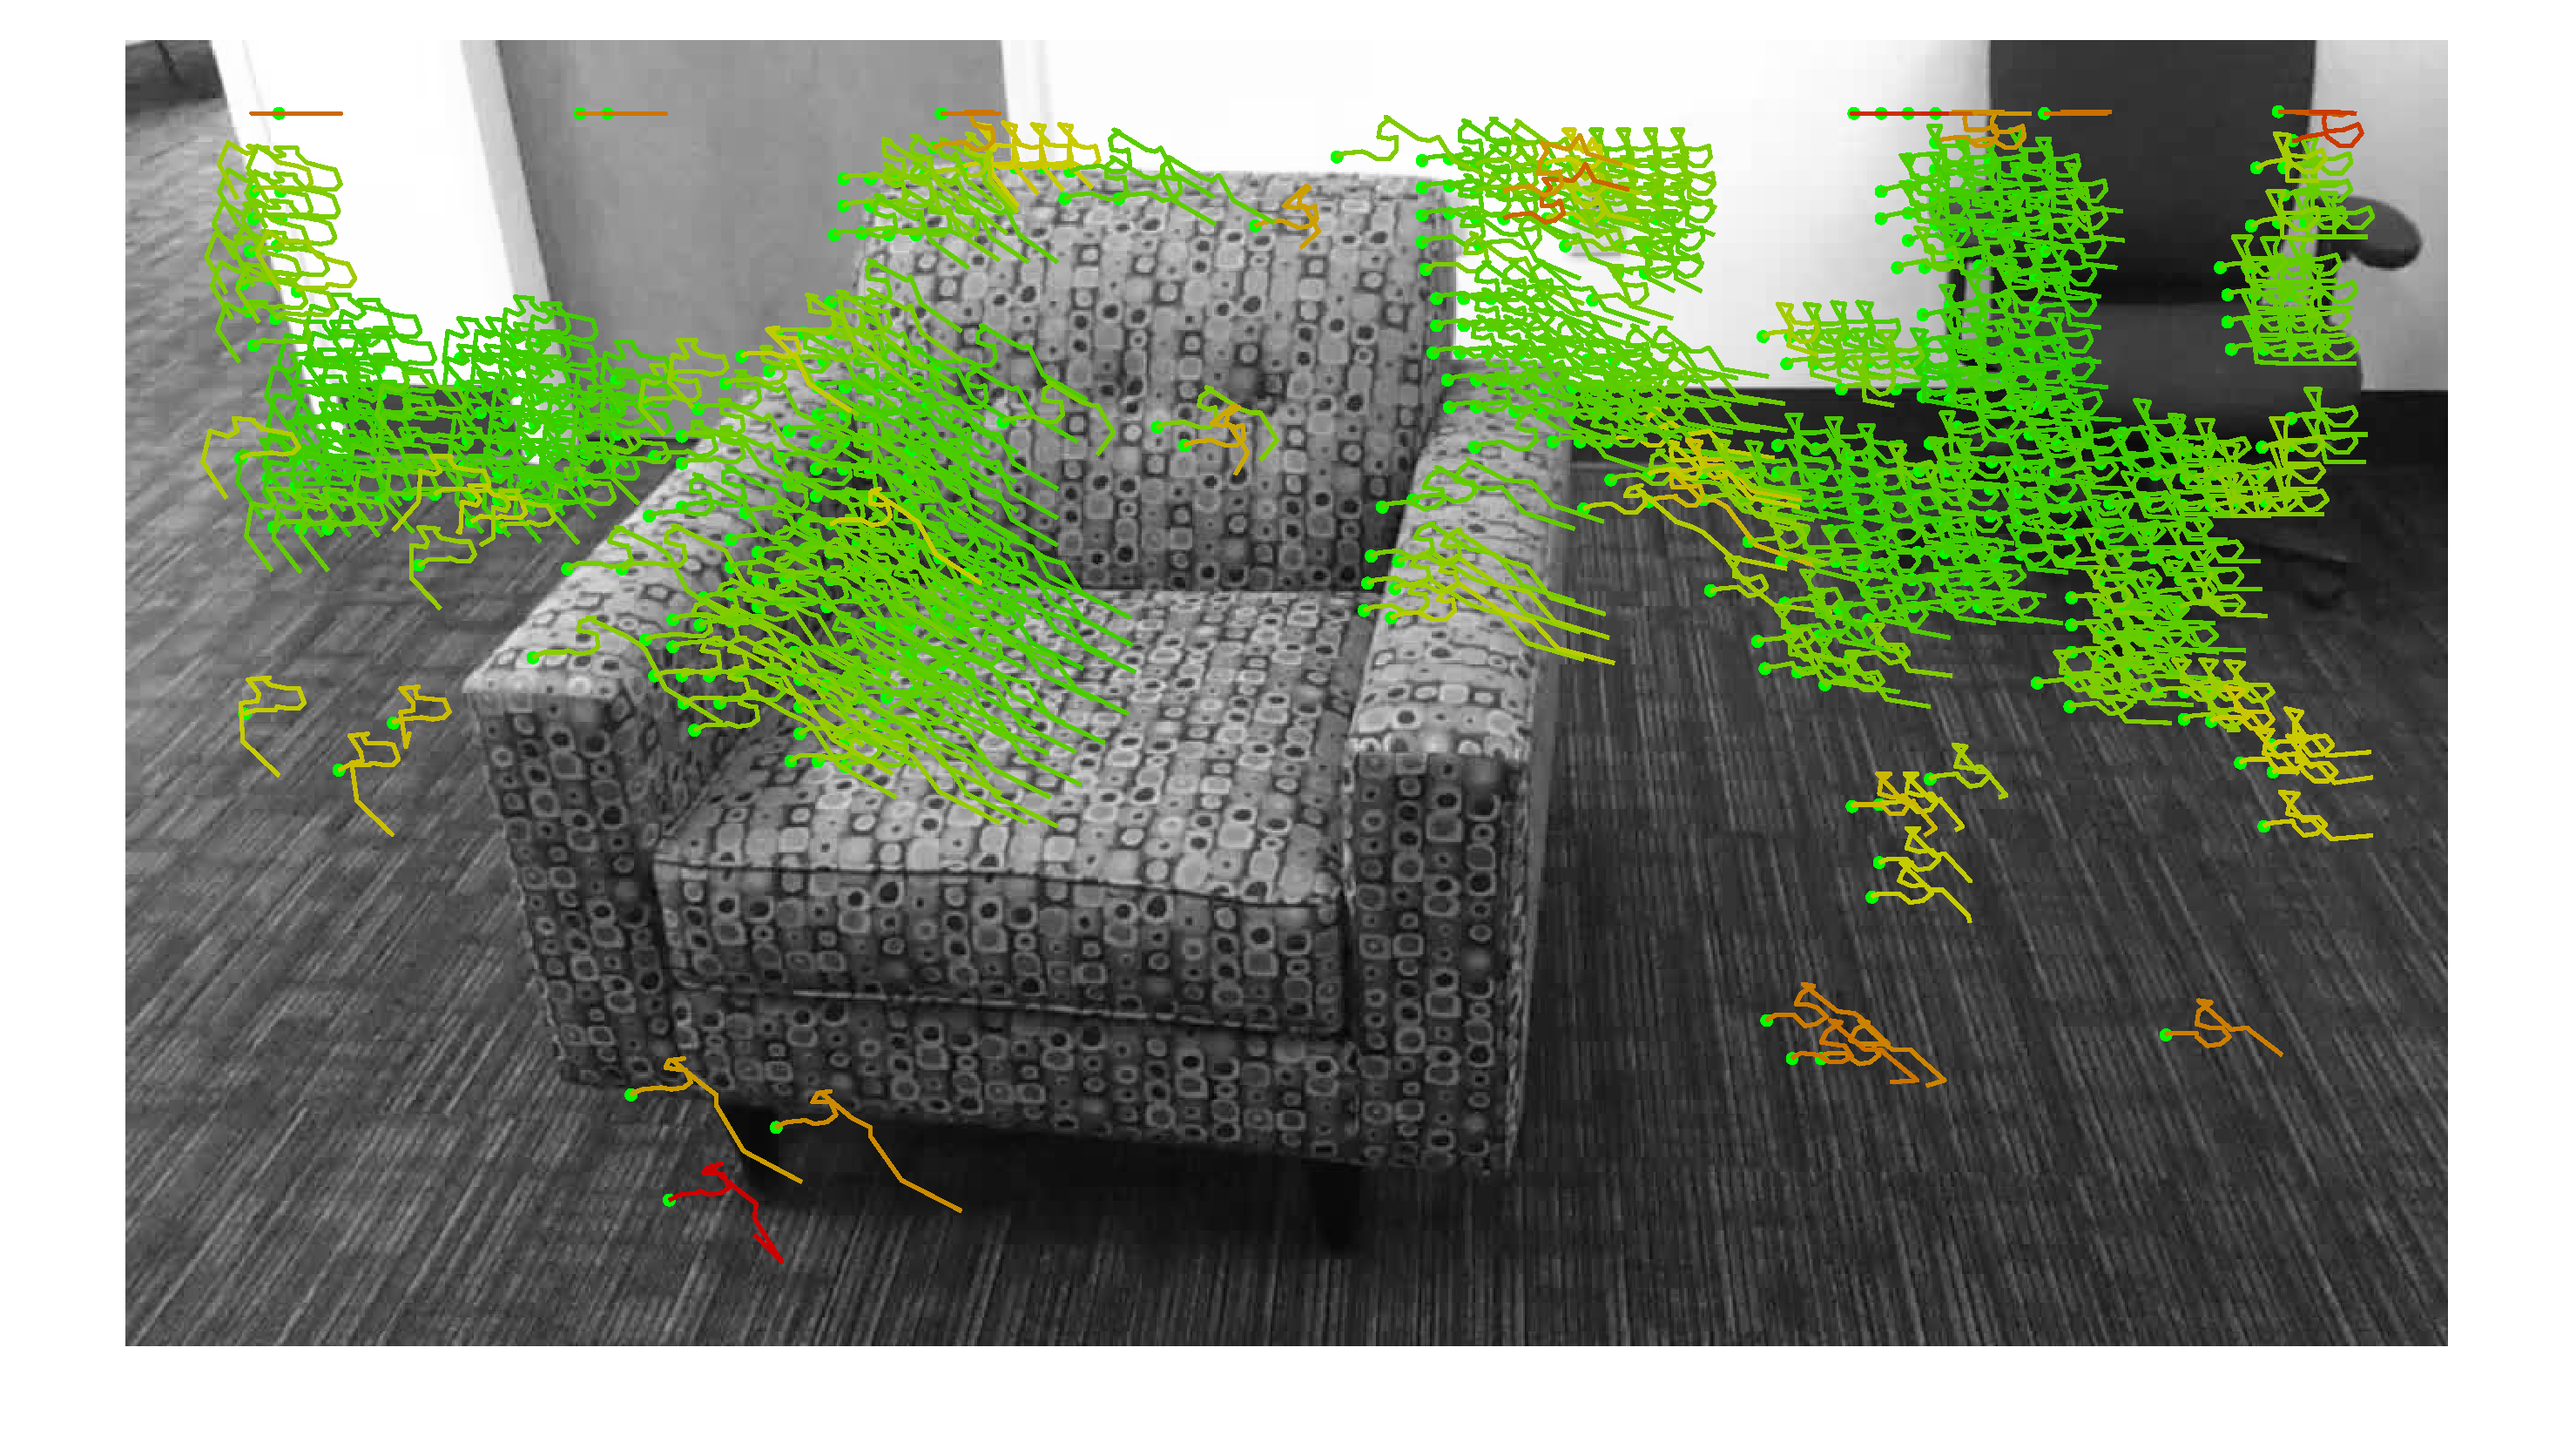
\includegraphics[width=3in]{figs/lounge-1.pdf} \\ (b)
			%\caption{default}
		\end{minipage}
		\vspace{0.1cm}
		\begin{minipage}[b]{\linewidth}
			\centering
			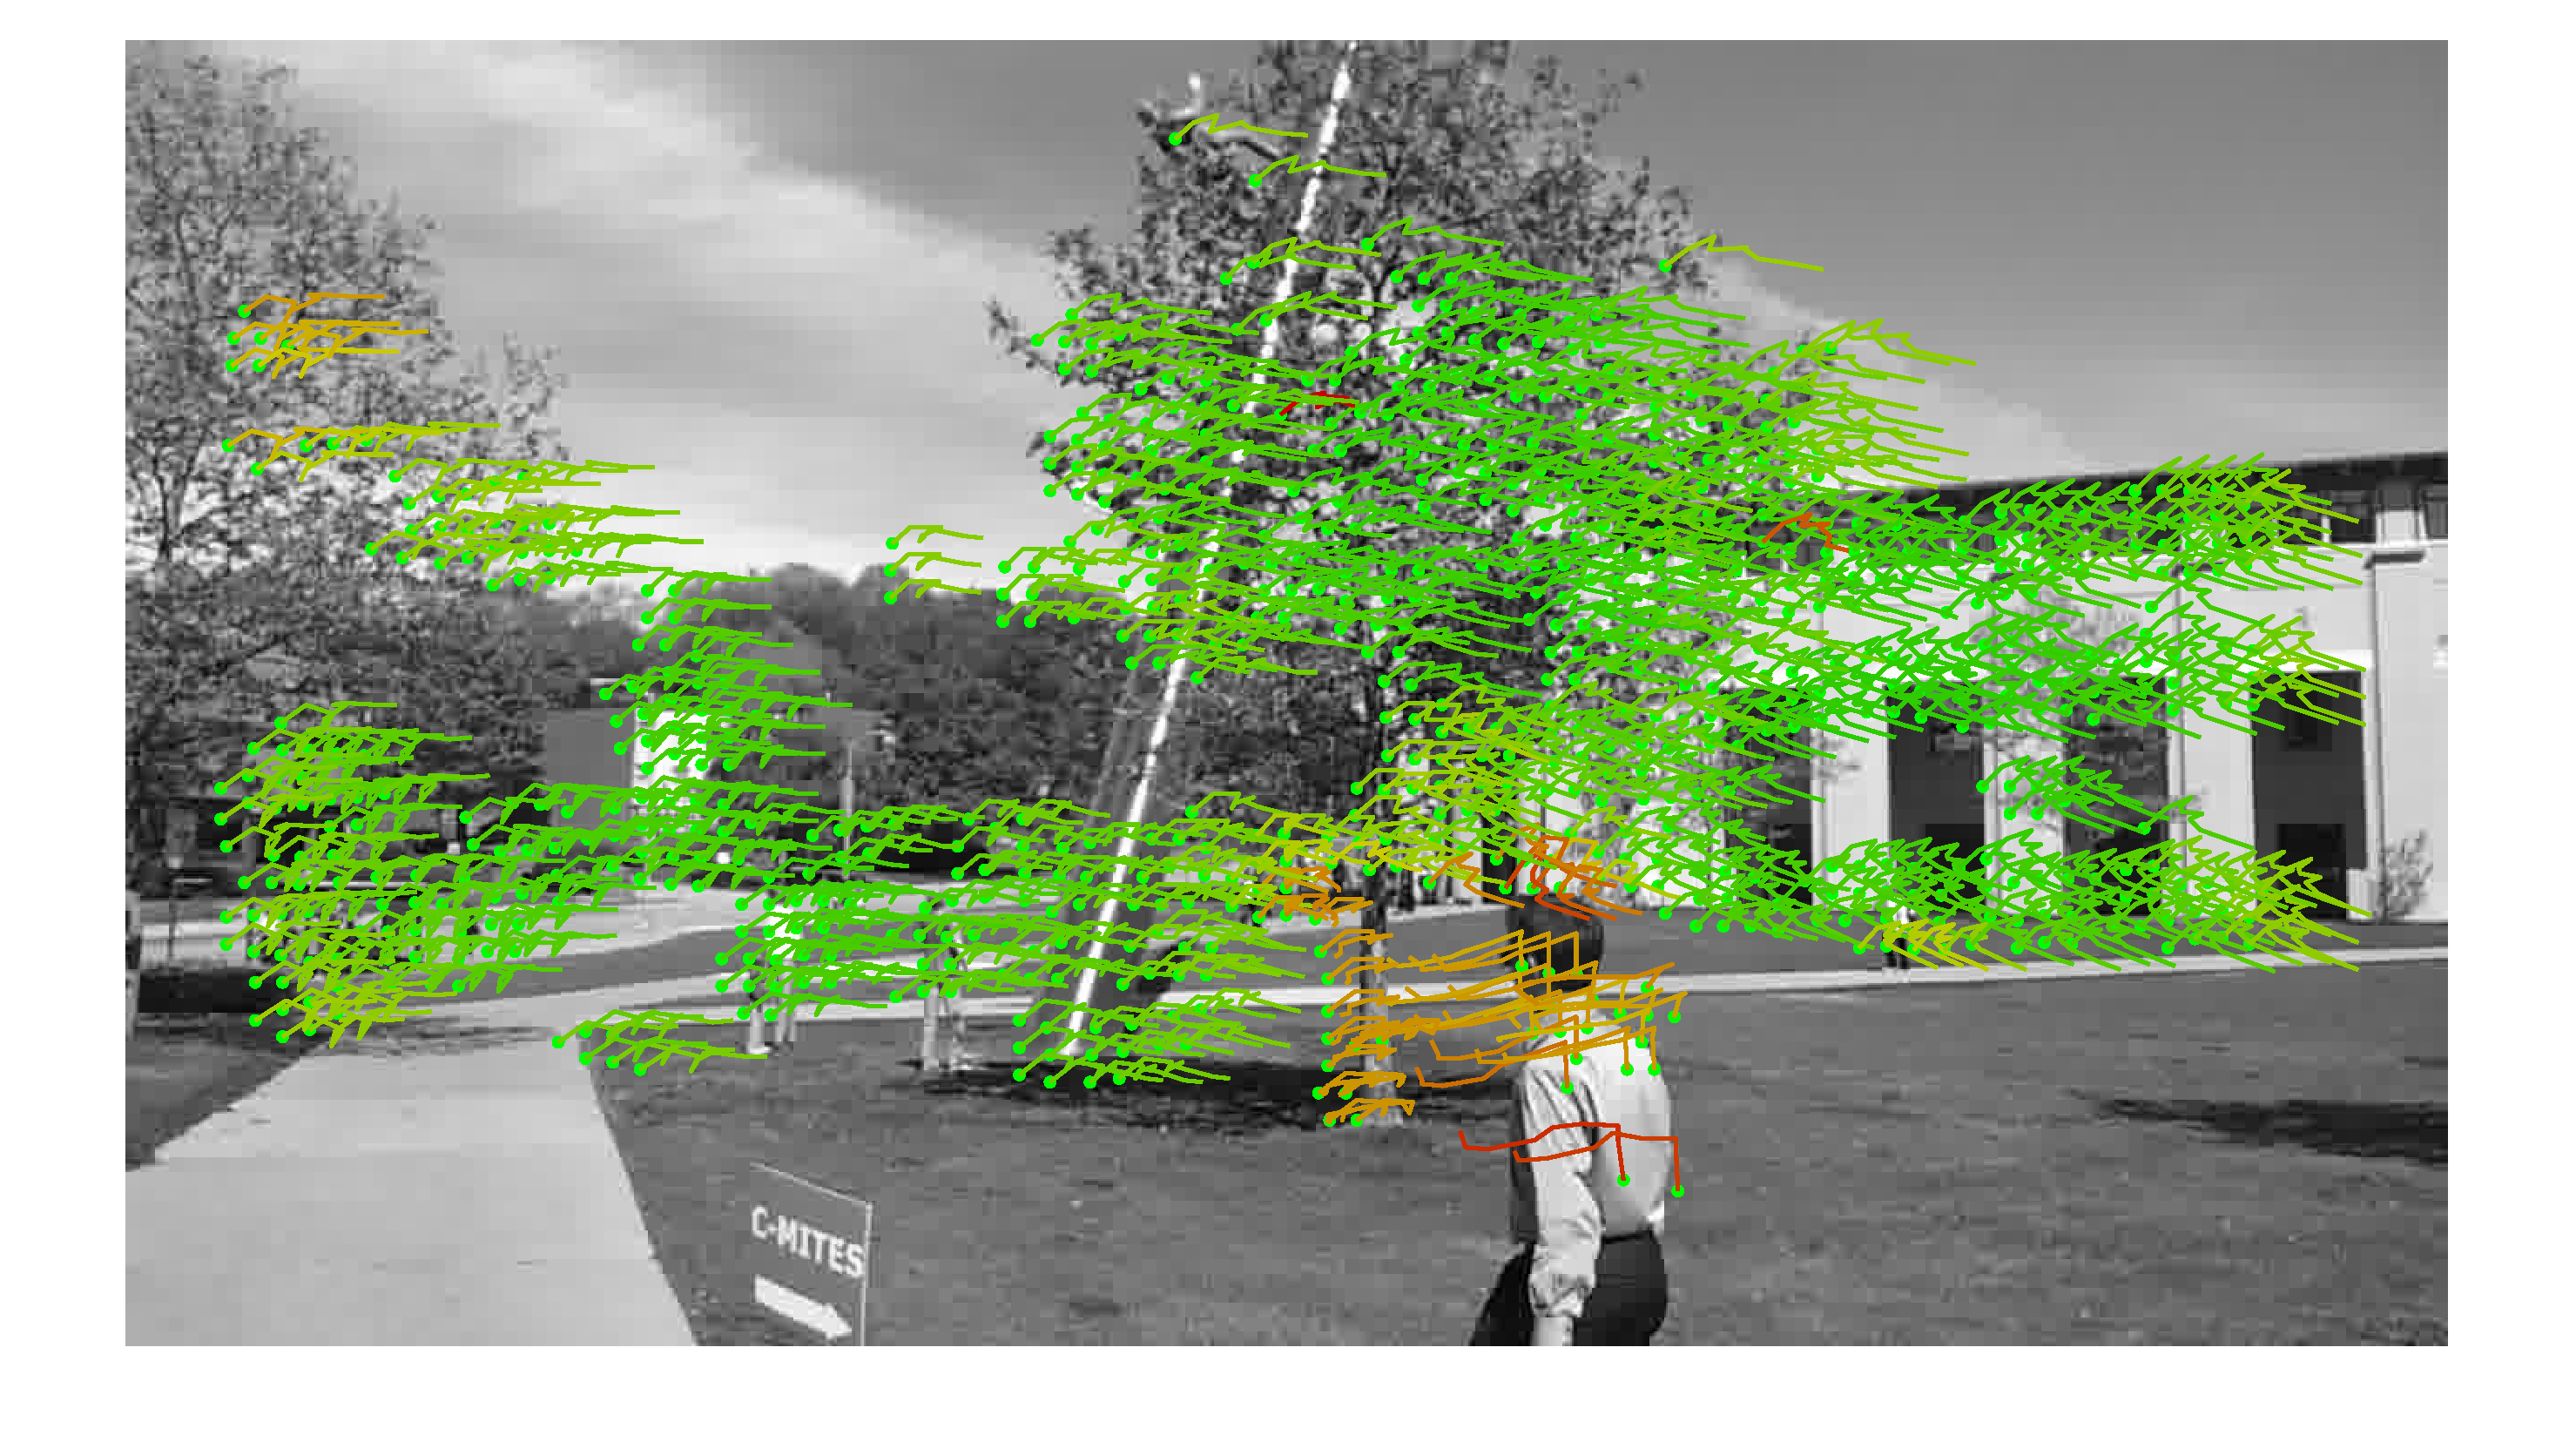
\includegraphics[width=3in]{figs/outdoor3-90.pdf} \\ (c)
			%\caption{default}
		\end{minipage}

	\end{minipage}
	\caption{Traces colored by GMM score for (a) desk chair, (b) lounge chair, and (c) outdoors.  Green reflects a high GMM score and red reflects a low GMM score.}
	\label{fig:colored-traces}
\end{figure}


In addition to visually evaluating the success of our algorithm in isolating
outlier traces, we compared the purity score of the data before and after
outlier removal.  In running our algorithm and evaluation across all four data
sets, we found that in every case outlier removal improved the purity score and
thus structure from motion result.  The purity score comparison can be seen in
Table \ref{tab:purities}.  Not surprisingly, the algorithm seems to be most
useful when there is a moving object in the scene, as this results in a large
number of outlier points that would disrupt the structure from motion
algorithm.  Overall, we considered our method to work as intended and improved
the resulting structure from motion.

\begin{table}[tb]
	\begin{center}
		\begin{tabular}{|l|c|c|}
			\hline
			\multirow{2}{*}{Data Set}  &\multicolumn{2}{|c|}{Purity Score}\\ \cline{2-3}
			& \multicolumn{1}{|c|}{Original}  & \multicolumn{1}{|c|}{With Outlier Removal}\\ \hline
			Desk Chair & 36.14 & 40.63 \\ \hline
			Lounge Chair & 89.2 & 111.36 \\ \hline
			Outdoors & 90.43 & 175.44 \\ \hline
			Outdoors 2 & 96.37 & 127.96 \\ \hline
		\end{tabular}
	\end{center}
	\caption{Comparison of Purity Score before and after outlier removal.}
	\label{tab:purities}
\end{table}


% subsection Experiments (end)


\section{Robust Motion Isolation} 

As discussed previously, our Gaussian mixture model does an excellent job of
distinguishing traces of moving objects from traces of static objects caused
only by the motion of the camera (regardless of the camera motion).  We decided
to apply this aspect of our model to the task of isolating motion in a scene,
regardless of unstable video footage.  We first describe the model we use to
take traces and corresponding GMM probabilities and create a video with only the
moving elements.  We then describe the experiments and results of our
implementation.

\subsection{Model Application} % (fold)
\label{sub:Model Application}

\paragraph{Traces to Frames} % (fold)
\label{par:Traces to Frames}

Our problem can be formulated as follows: Given a set of traces and the GMM
probability for each, we look to find the probability that pixel $\pi_j =
(x_j,y_j)$ at time $t$ is of a moving object in the scene or not.  In order to
calculate this we first transform a few parameters.  First, we invert and bound
the range of GMM probabilities to create a \alex{movement} score.  Given ${\bf
P}$ is the vector of log-probabilities returned by the GMM for a given set of
traces, we create the following vector of movement scores:
\begin{align}
	{\bf s} = - \frac{ {\bf P} - {\rm max}({\bf P}) }{ {\rm min}({\bf P}) }
\end{align}
Under this transformation, the scores are bounded to the range 0 to 1 such that
traces with a high probability of being outliers, and thus movement, are close
to 1, and those that are not are closer to 0.

With this score, we can create a probabilistic model for any given pixel being
of a moving object or not.  In our model we assume independence among both
pixels and traces.  Therefore, given score $s_i$ for trace $T_i$, at position
$(x_{i,t},y_{i,t})$ at time $t$, we claim the following probabilities:
\begin{align}
	P(s_i,x_{i,t},y_{i,t}|{\rm pixel}_j = {\it moving})  &= \frac{1}{1 + e^{-\gamma(s_i - \beta)}} e^{- \frac{|(x_{i,t},y_{i,t}) - \pi_j|^2}{\alpha_1}}
	\\ P(s_i,x_{i,t},y_{i,t}|{\rm pixel}_j = {\it static})  &= \left( 1 - \frac{1}{1 + e^{-\gamma(s_i - \beta)}}\right) e^{- \frac{|(x_{i,t},y_{i,t}) - \pi_j|^2}{\alpha_2}}
\end{align}
The first term in each probability puts the movement score through the logistic
function in order to partition scores into being generally very close to zero
(most likely static) or very close to one (most likely moving).  For this
logistic function we have two parameters: $\beta$ and $\gamma$.  $\beta$ we
pick as some threshold score for which scores less than the threshold are
pushed to 0 and scores greater than the threshold are pushed to one.  Picking
this threshold is similar to the problem of picking the threshold for the
structure for motion problem.  While this could be done dynamically based on an
analysis of the score distribution, similar to that in Figure
\ref{fig:logpdfs}, we generally used a threshold at about the 75th percentile
mark to separate the scores.  (Remember that scores are inverted such that high
scores are more likely to be of moving objects.)  The parameters $\gamma$ is
used to push values toward zero or one and leave few values near 0.5; we set
$\gamma = 100$.

The second term is \alex{of the form of a Gaussian} using the distance between
the feature and the pixel to determine what influence the feature's score has
on the probability for the pixel.  The terms $\alpha_1$ and $\alpha_2$
determine the \alex{width} of the Gaussian.  With this function we make sure
that features closer to a pixel have a stronger influence on their probability
than pixels far away.  We also set, based on experimentation, $\alpha_1 =
2\alpha_2$ so that features that appear be moving having a wider range of
influence than those that do not.


Given these probabilities for trace scores conditional on pixel movements, we
can calculate the general probability of a pixel being of a moving or static
object, following Bayes rule
\begin{align}
	P({\rm pixel}_j = o|{\bf s},W) = \frac{ P({\bf s},W|{\rm pixel}_j = o) P({\rm pixel}_j = o) }{ P({\bf s}, W) },
\end{align}
where $o \in \{ {\it moving}, {\it static} \}$.  We make the assumption that we
have no priors on pixels nor traces.  Also, because under our model we assume
independence among traces, we can simplify our calculation to the following equation
\begin{align}
	\log P({\rm pixel}_j = o|{\bf s},W) = \sum_i \log P(s_i,x_{i,t},y_{i,t}|{\rm pixel}_j = o) \label{eq:logsum}
\end{align}
At the of the calculation, if $P({\rm pixel}_j = {\it moving}|{\bf s},W) > P({\rm
pixel}_j = {\it static}|{\bf s},W)$ then we consider the pixel to be of a moving object,
and if not we consider it to be static.  Doing this for all pixels in each
frame, we can construct a video isolating only the moving elements.

\alex{is there a way to weave ``expectation maximization'' into this?}
\alex{verify equations above - a bit sketchy}

% paragraph Traces to Frames (end)

\paragraph{Trace Sets} % (fold)
\label{par:Trace Sets}

One key challenge we found in performing feature tracking was that features
were often lost if tracked over many frames.  In the case of motion
isolation, we do not care so much if any given feature is tracked continuously,
but rather just if each pixel is more likely to be of a moving or static
object.


\newcommand{\fset}{ \EuScript{F} }
\newcommand{\fstep}{ f_s }
\newcommand{\fwin}{ f_w }

Therefore, to minimize losing features and for each frame have more tracked
features, we break the video into shorter sets of frame, each frame set denoted by
$\fset_k$.  \alex{In order to keep some of the elements of tracking across the video},
we have some overlap between frame sets, which we denote as frame step
$\fstep$.  Therefore, the first frame of $\fset_k$ is $\fstep$ frames after the
first frame of $\fset_{k-1}$. Frame sets have a window size $\fwin$, such that
they contain a total of $\fwin\fstep$ frames, or alternatively, each frame is
part of $\fwin$ frame sets.
(In practice we set $\fwin = 3$ and $\fstep = 3$ or 5.)

Given such a set up, we can run our previously described algorithm, calculating
the GMM, movement scores, and pixel movement probabilities for each frame set.
Because we assume independence among traces, we can simply include the
log-probabilities for each frame set together in the sum in Equation
\eqref{eq:logsum}, leaving us still with the final comparison $P({\rm pixel}_j
= {\it moving}|{\bf s},W) > P({\rm pixel}_j = {\it static}|{\bf s},W)$ to
determine if a pixel is more likely to be of a moving object or not.

% paragraph Trace Sets (end)



% subsection Model Application (end)

\subsection{Experiments} % (fold)
\label{sub:Experiments}


\paragraph{Setup} % (fold)
Our implementation followed the algorithm given above fairly closely, and only
required adjusting parameters slightly depending on some unique video features
like image resolution.  As there was no simple ground truth, we largely
evaluated our results based on the quality of the movie produced.  We ran our
algorithm on a number of different data sets: two videos collected with an Android
mobile phone of the authors walking around a computer lab and two
\alex{home-shot}, low quality videos downloaded from YouTube.  For each we
selected a subset of the video to run our algorithm over.  In each frame,
pixels that were more likely to be of static objects than moving objects were
removed, leaving only the ``moving pixels.''  The results are discussed below.

\alex{do we want to put in parameters we chose here, or leave them weaved in
above: $\gamma$, $\beta$, $\alpha_1$, $\alpha_2$, $\fstep$, $\fwin$.}

% paragraph Setup (end)

\paragraph{Results} % (fold)
\label{par:Results}

Overall, the algorithm ran as desired.  In each video we generally isolate the
parts of the scene that are moving.  Figure \ref{fig:alex-walking} gives an
example of the steps of the process for a video of Alex walking through the
lab.  We see the video generally captures where he is and removes the
background.

\begin{figure}[tb]
	\centering
	\begin{subfigure}[b]{0.33\textwidth}
		\centering
		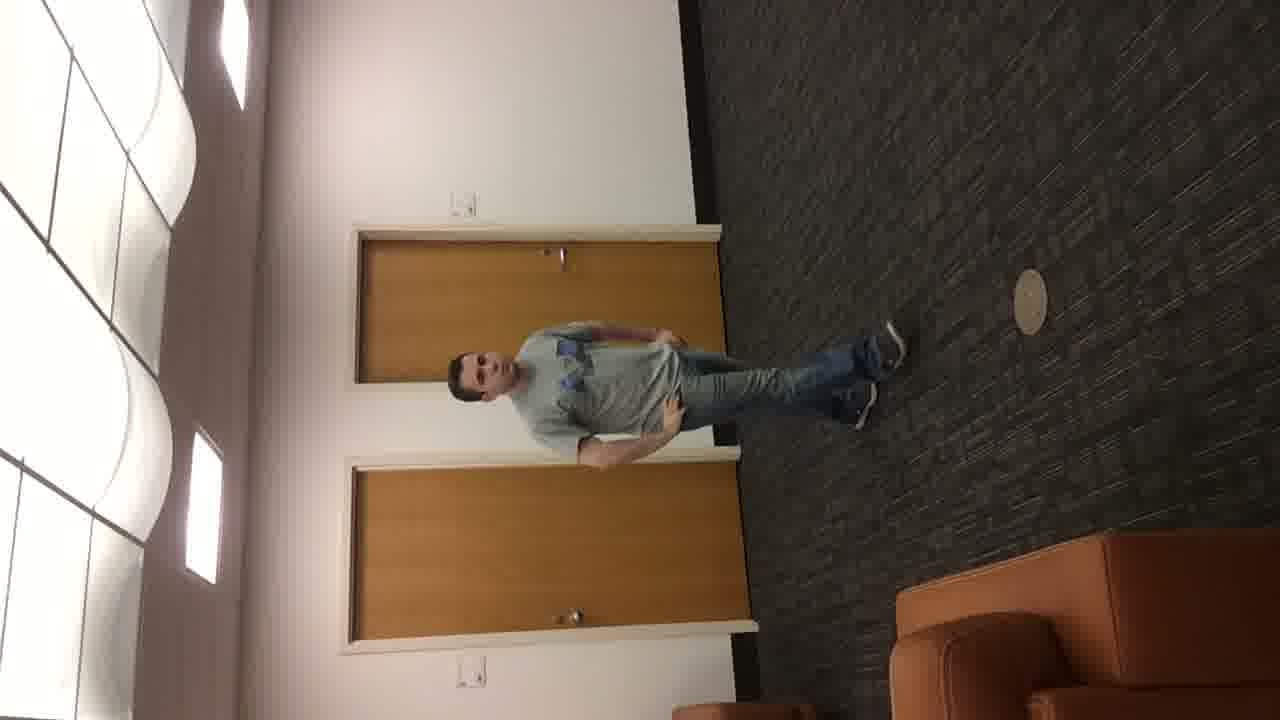
\includegraphics[width=3in,angle=-90]{figs/alex-image30.jpg}
		\caption{Single frame before analysis.}
	\end{subfigure}%
	\begin{subfigure}[b]{0.33\textwidth}
		\centering
		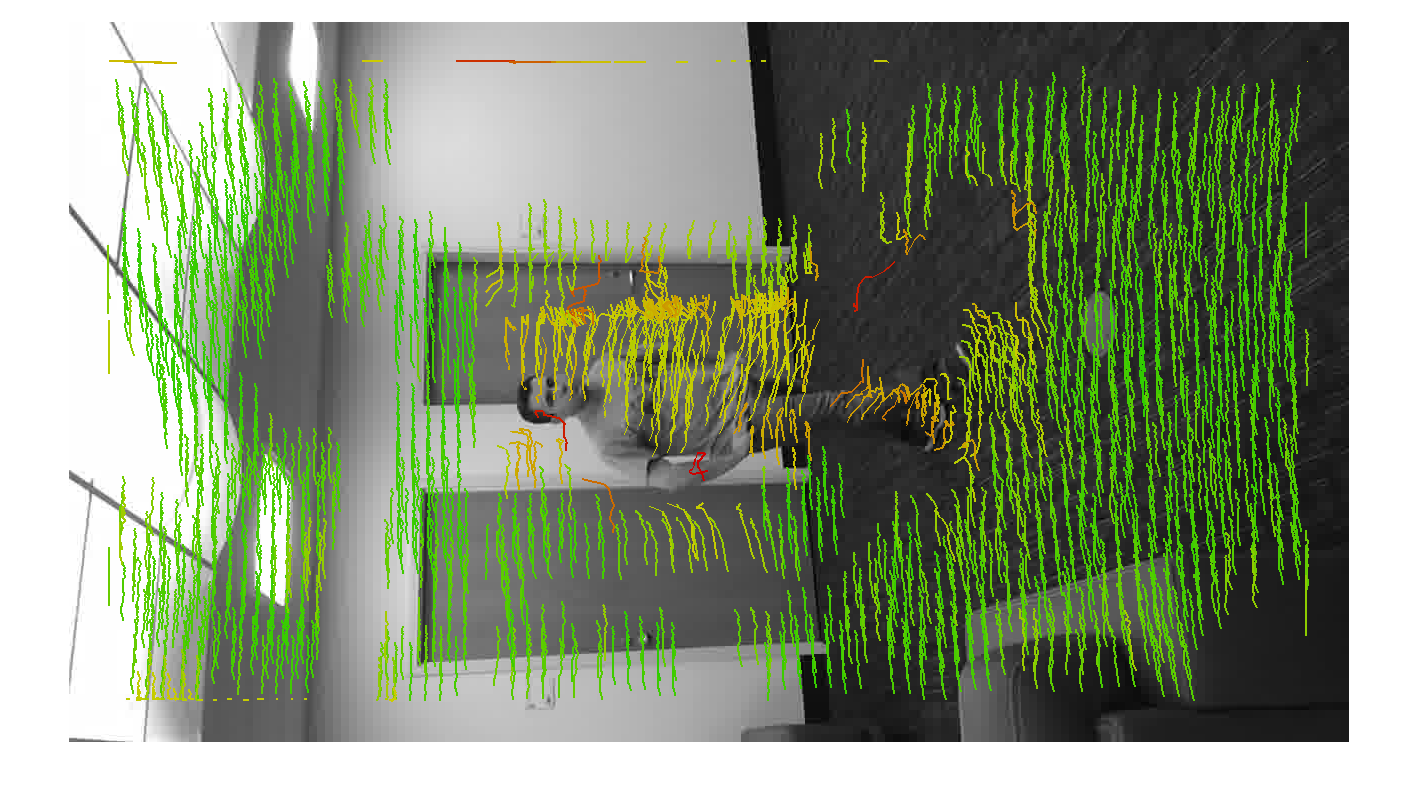
\includegraphics[width=3.2in,angle=-90]{figs/gmm-motion.png}
		\caption{Traces with by GMM probability}
	\end{subfigure}%
	\begin{subfigure}[b]{0.33\textwidth}
		\centering
		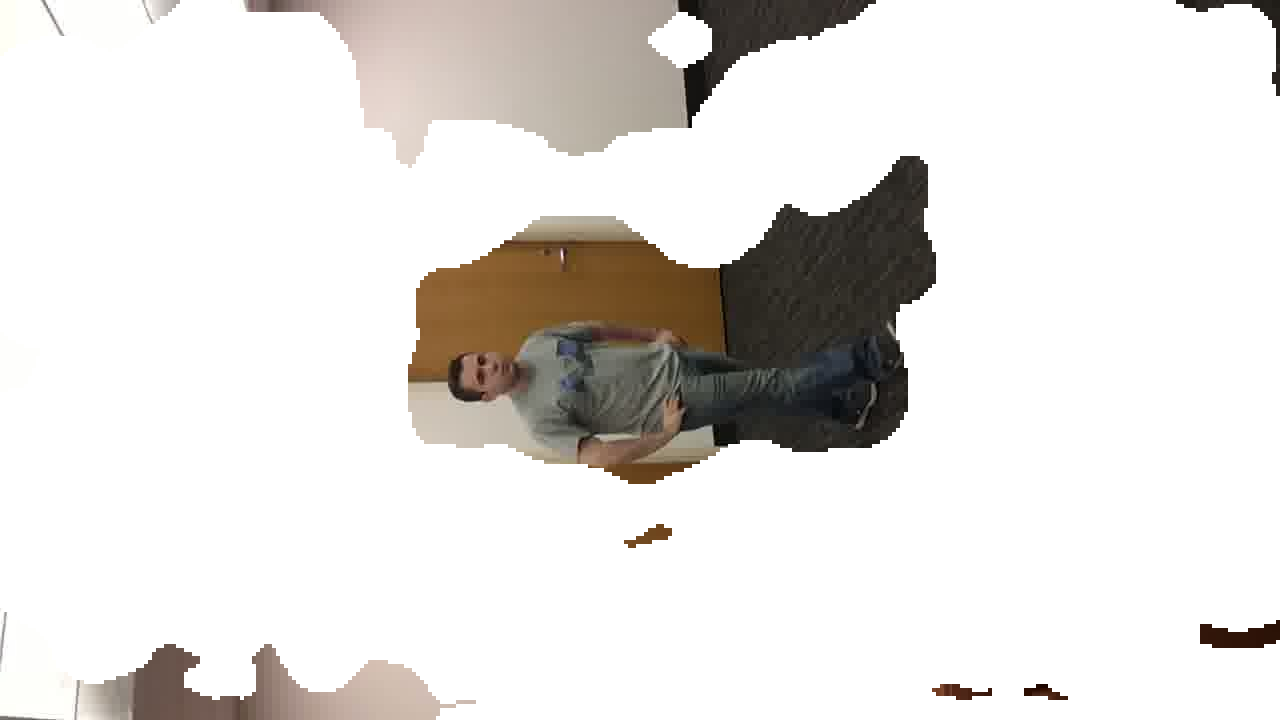
\includegraphics[width=3in,angle=-90]{figs/alex30.png}
		\caption{Frame after motion isolation}
	\end{subfigure}%

	\caption{Step through of our algorithm running on video we took of Alex walking.}
	\label{fig:alex-walking}
\end{figure}

In practice we found that videos of dancing we're excellent examples as the
motion of the person was {\it very} different from the motion of the
background.  On YouTube we found two famous videos of dancing: ``Bimbo Dancer''
and ``Break Dance kick.''  Both videos are relatively low quality with a shaky
camera, but our algorithm performs well.  In Figure \ref{fig:bimbodance} we see
a baby dancing on a table, and the algorithm successfully picks out his traces
as unique from those in the background.

\begin{figure}[tb]
	\centering
	\begin{subfigure}[b]{0.33\textwidth}
		\centering
		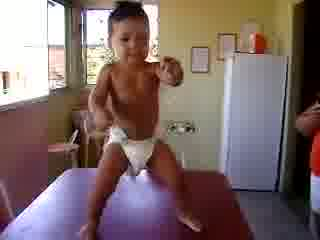
\includegraphics[width=0.9\textwidth]{figs/bimbodance-image50.jpg}
		\caption{Single frame before analysis.}
	\end{subfigure}%
	\begin{subfigure}[b]{0.33\textwidth}
		\centering
		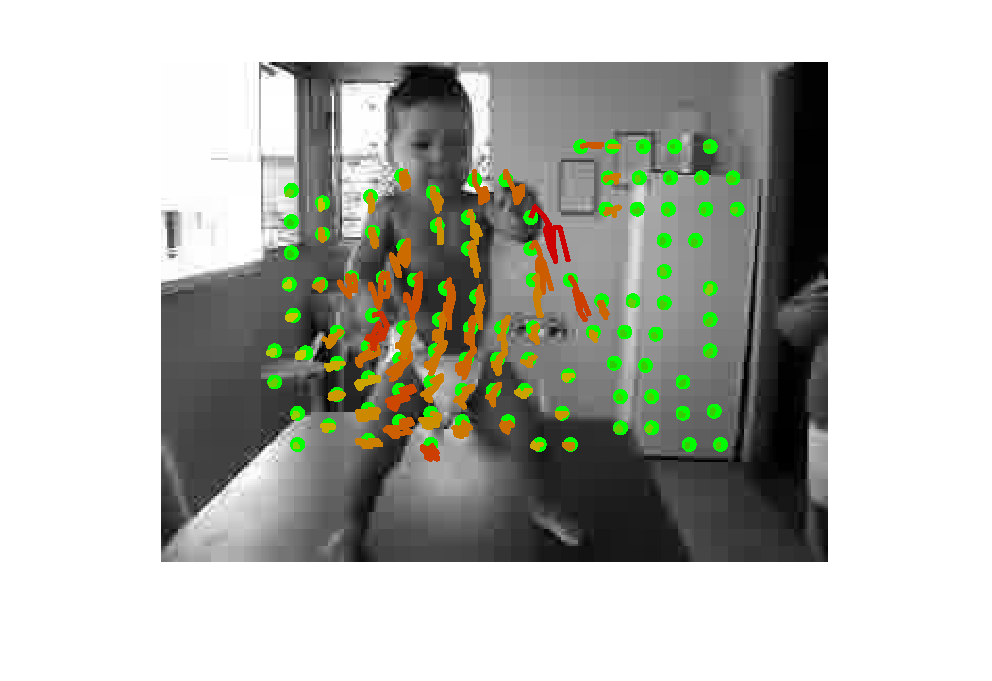
\includegraphics[width=1.2\textwidth]{figs/bimbodance-50.eps}
		\caption{Traces with by GMM probability}
	\end{subfigure}%
	\begin{subfigure}[b]{0.33\textwidth}
		\centering
		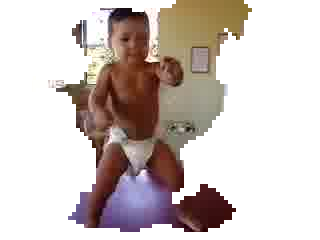
\includegraphics[width=0.9\textwidth]{figs/bimbodance-image50.png}
		\caption{Frame after motion isolation}
	\end{subfigure}%

	\caption{Step through of our algorithm running on video of a baby dancing.}
	\label{fig:bimbodance}
\end{figure}

Complete videos of the output can be found online at \alex{INSERT URL HERE}.
Overall we were pleased with the result, though we believe fine-tuning the
parameters of the model could improve the output.  We also believe that
combining this information with computer vision techniques, such as image
segmentation, could produce much more robust results.


% paragraph Results (end)



% subsection Experiments (end)


\section{Conclusion} 

%\subsubsection*{References}

%References follow the acknowledgments. Use unnumbered third level heading for
%the references. Any choice of citation style is acceptable as long as you are
%consistent. It is permissible to reduce the font size to `small' (9-point) 
%when listing the references. {\bf Remember that this year you can use
%a ninth page as long as it contains \emph{only} cited references.}


{% \small
\bibliographystyle{abbrv}
\bibliography{bib}
}

%\small{
%[1] Alexander, J.A. \& Mozer, M.C. (1995) Template-based algorithms
%for connectionist rule extraction. In G. Tesauro, D. S. Touretzky
%and T.K. Leen (eds.), {\it Advances in Neural Information Processing
%Systems 7}, pp. 609-616. Cambridge, MA: MIT Press.

%[2] Bower, J.M. \& Beeman, D. (1995) {\it The Book of GENESIS: Exploring
%Realistic Neural Models with the GEneral NEural SImulation System.}
%New York: TELOS/Springer-Verlag.

%[3] Hasselmo, M.E., Schnell, E. \& Barkai, E. (1995) Dynamics of learning
%and recall at excitatory recurrent synapses and cholinergic modulation
%in rat hippocampal region CA3. {\it Journal of Neuroscience}
%{\bf 15}(7):5249-5262.
%}

\end{document}
